\documentclass[12pt,a4paper,oneside]{report}

\usepackage[margin=1in]{geometry}
\usepackage{setspace}
\usepackage{graphicx}
\usepackage{float}
\usepackage{array}
\usepackage{booktabs}
\usepackage{longtable}
\usepackage{tabularx}
\usepackage{multirow}
\usepackage{enumitem}
\usepackage{amsmath}
\usepackage{amssymb}
\usepackage{fancyhdr}
\usepackage{xcolor}
\usepackage{hyperref}
\usepackage{caption}
\usepackage{tikz}
\usepackage{titlesec}
\usepackage{url}
\usepackage{mathptmx}

\usetikzlibrary{arrows.meta,positioning,shapes.geometric,shapes.multipart,fit,calc,backgrounds}

\hypersetup{
  colorlinks=true,
  linkcolor=black,
  urlcolor=blue,
  citecolor=black,
  pdftitle={E-Assistant: AI-Powered Product Search Agent},
  pdfauthor={Student Name 1 and Student Name 2}
}

\linespread{1.213}\selectfont
\setlength{\parindent}{0.5in}
\setlength{\parskip}{4pt}
\setlength{\extrarowheight}{6.5pt}
\captionsetup{font=small}
\setlength{\LTleft}{0pt}
\setlength{\LTright}{0pt}
\raggedbottom

\pagestyle{fancy}
\fancyhf{}
\fancyfoot[C]{\thepage}
\renewcommand{\headrulewidth}{0pt}

\renewcommand{\contentsname}{TABLE OF CONTENTS}
\renewcommand{\listfigurename}{LIST OF FIGURES}
\renewcommand{\listtablename}{LIST OF TABLES}

\newcolumntype{Y}{>{\raggedright\arraybackslash}X}
\newcolumntype{L}[1]{>{\raggedright\arraybackslash}p{#1}}
\newcolumntype{C}[1]{>{\centering\arraybackslash}p{#1}}

\newcommand{\projecttitle}{E-Assistant: AI-Powered Product Search Agent}
\newcommand{\studentone}{Amman Zarkash}
\newcommand{\studentoneid}{FA22-BAI-019}
\newcommand{\studenttwo}{Muhammad Umar}
\newcommand{\studenttwoid}{FA22-BAI-041}
\newcommand{\supervisorname}{Dr. Zahoor Tanooli}

\newcommand{\uitwoscreenshots}[2]{
\begin{figure}[p]
\centering
\includegraphics[width=0.99\textwidth,height=0.47\textheight,keepaspectratio]{#1}\\[0.02\textheight]
\includegraphics[width=0.99\textwidth,height=0.47\textheight,keepaspectratio]{#2}
\end{figure}
\clearpage
}

\begin{document}

\pagenumbering{gobble}

\begin{titlepage}
\centering
\vspace*{0.2cm}
{\LARGE \textbf{COMSATS University Islamabad}}\\[0.15cm]
{\large Attock Campus}\\[0.35cm]

\includegraphics[height=2.4cm]{comsats.jpg}\\[0.35cm]
{\Large \textbf{Final Year Project Documentation}}\\[0.35cm]
{\large for}\\[0.25cm]
{\Large \textbf{\projecttitle}}\\[0.55cm]
{\large by}\\[0.25cm]
{\large \studentone}\\[0.1cm]
{\normalsize \studentoneid}\\[0.25cm]
{\large \studenttwo}\\[0.1cm]
{\normalsize \studenttwoid}\\[0.55cm]
{\large Supervised by}\\[0.15cm]
{\large \supervisorname}\\[0.55cm]
{\large Bachelor of Science in Artificial Intelligence}\\
{\large Department of Computer Science}\\[0.15cm]
{\large 2022--2026}\\[0.35cm]
{\large Spring 2026}
\end{titlepage}

\begin{titlepage}
\centering
\vspace*{1cm}
{\LARGE \textbf{\projecttitle}}\\[1cm]
{\large This project documentation is submitted to the Department of Computer Science,}\\
{\large COMSATS University Islamabad, Attock Campus, in partial fulfillment}\\
{\large of the requirements for the degree of BS in Artificial Intelligence.}\\[1.3cm]

\begin{tabular}{ll}
\textbf{Name} & \textbf{Registration Number} \\
\studentone & \studentoneid \\
\studenttwo & \studenttwoid \\
\end{tabular}\\[1.5cm]

\textbf{Supervisor}\\[0.3cm]
\supervisorname\\
Department of Computer Science\\
COMSATS University Islamabad, Attock Campus\\[1.5cm]

{\large April 2026}
\end{titlepage}

\begin{titlepage}
\centering
\vspace*{1cm}
{\LARGE \textbf{Final Approval}}\\[1cm]
This project titled\\[0.4cm]
{\Large \textbf{\projecttitle}}\\[0.9cm]
submitted by\\[0.4cm]
\studentone\ (\studentoneid)\\
\studenttwo\ (\studenttwoid)\\[1cm]
has been reviewed and approved for submission to COMSATS University Islamabad, Attock Campus.\\[1.5cm]

\begin{flushleft}
\textbf{External Examiner:} \hrulefill\\[1.0cm]
\textbf{Supervisor:} \hrulefill\\[0.2cm]
\hspace*{2.4cm}\supervisorname\\[1.0cm]
\textbf{Head of Department:} \hrulefill\\[0.2cm]
\hspace*{4cm}Head of Department
\end{flushleft}
\end{titlepage}

\begin{titlepage}
\centering
\vspace*{1cm}
{\LARGE \textbf{Author's Declaration}}\\[1cm]
\begin{spacing}{1.35}
We, \studentone\ (\studentoneid) and \studenttwo\ (\studenttwoid), declare that the work presented in this documentation is our own work carried out during the scheduled final year project period for the project titled \textbf{\projecttitle}. Wherever the words, ideas, figures, or findings of other authors have been used, they have been appropriately acknowledged through references. To the best of our knowledge, this document does not contain plagiarized material beyond the acceptable academic limit.
\end{spacing}

\vfill
\begin{flushleft}
\textbf{Student Signature:} \hrulefill\\[0.6cm]
\textbf{Student Signature:} \hrulefill\\[0.6cm]
\textbf{Date:} \hrulefill
\end{flushleft}
\end{titlepage}

\begin{titlepage}
\centering
\vspace*{1cm}
{\LARGE \textbf{Certificate}}\\[1cm]
\begin{spacing}{1.35}
It is certified that \studentone\ (\studentoneid) and \studenttwo\ (\studenttwoid) have completed the work described in this report under my supervision at the Department of Computer Science, COMSATS University Islamabad, Attock Campus. In my opinion, the work fulfills the academic requirements for submission of the BS Artificial Intelligence final year project documentation.
\end{spacing}

\vfill
\begin{flushleft}
\textbf{Supervisor:} \hrulefill\\[0.2cm]
\hspace*{2.6cm}\supervisorname\\
\hspace*{2.6cm}Department of Computer Science\\
\hspace*{2.6cm}COMSATS University Islamabad, Attock Campus\\[0.8cm]
\textbf{Head of Department:} \hrulefill
\end{flushleft}
\end{titlepage}

\begin{titlepage}
\centering
\vspace*{3cm}
{\Large \textbf{Dedicated to our parents, teachers, and all those}\\[0.3cm]
\textbf{who supported us throughout this project journey.}}
\end{titlepage}

\pagenumbering{roman}

\chapter*{ACKNOWLEDGEMENTS}
\addcontentsline{toc}{chapter}{ACKNOWLEDGEMENTS}
We are grateful to Allah Almighty for the guidance, patience, and opportunity to complete this work. We sincerely thank our supervisor, \supervisorname, for academic guidance, technical feedback, and continuous support throughout the design, implementation, and documentation of this project. The completion of this system required work across software engineering, machine learning, data processing, and interface design, and that work benefited directly from disciplined supervision.

We also acknowledge the support of the Department of Computer Science and COMSATS University Islamabad, Attock Campus, for providing an environment in which a practical AI product could be developed as more than a classroom prototype. The project integrates web scraping, ranking, conversational orchestration, database persistence, and frontend interaction into one coherent system, and that breadth reflects the training received during the degree program.

We are thankful to the open-source ecosystem as well. The implementation builds on several mature tools and frameworks, including FastAPI, MongoDB, React, Vite, Playwright, Beautiful Soup, Gradio, and sentence-transformer-based retrieval utilities. These technologies made it possible to focus on system integration, product behavior, and evaluation rather than reimplementing infrastructure from scratch.

Finally, we thank our families and friends for their patience during the long phases of experimentation, debugging, interface refinement, and report writing. Their support made it possible to carry the project from an idea into a working AI-assisted product-search platform.

\chapter*{Project Summary}
\addcontentsline{toc}{chapter}{Project Summary}
\textbf{\projecttitle} is an end-to-end AI product-search system designed to help a user search e-commerce offers through natural-language interaction and receive ranked product suggestions with follow-up support. The project combines indexed product retrieval, semantic matching, clustering, value-oriented ranking, live web fallback search, conversation memory, and a user-facing React interface under the single product identity \textbf{E-Assistant}.

The implementation is organized around four major runtime parts. First, a React/Vite frontend provides the user experience for search, result browsing, follow-up conversation, history restoration, and an informational about page. Second, a FastAPI backend exposes search, recommendation, assistant, interaction-logging, metrics, and labeling endpoints. Third, an assistant orchestration layer manages conversational intent, context continuity, clarification handling, comparison flow, refinement flow, and selected-product follow-ups. Fourth, a data and ranking layer stores normalized offers in MongoDB and processes them through text retrieval, semantic matching, clustering, reranking, and collaborative-filtering-based personalization.

The assistant does not act as a free-text chatbot alone. It uses an internal MCP-style tool server that exposes operational tools such as indexed offer search, live web product search, direct page inspection, offer detail retrieval, and interaction logging. This makes the system traceable: conversational responses are grounded in tool results rather than invented store data. When indexed results are weak or follow-up information is missing, the system can inspect product pages and search live web sources before answering.

The resulting system demonstrates how an AI assistant can be embedded in a realistic commerce workflow rather than presented as an isolated language model demo. It is not only a search engine and not only a chat interface. It is a multi-component product-search application with data ingestion, ranking, conversation management, persistence, and interface support. This documentation explains that implemented system in terms of requirements, architecture, data design, UI behavior, runtime algorithms, and deployment.

\tableofcontents
\listoffigures
\listoftables

\clearpage
\pagenumbering{arabic}

\chapter{Introduction}

This chapter introduces \textbf{\projecttitle} as a complete AI product rather than a standalone search script or model demo. The project addresses the practical problem of finding relevant, high-value products across e-commerce sources while preserving conversational continuity, traceability, and deployment realism. It combines indexed retrieval, live web support, ranking logic, interface workflows, and persistent conversation state into one implemented system.

\section{Introduction}
Online product search has a familiar weakness: the user can easily find thousands of listings, but turning those listings into a reliable decision still requires manual effort. A typical buyer must jump between stores, compare prices, inspect ratings, check availability, verify delivery conditions, and remember earlier results while refining the search. The practical problem is therefore not only retrieval. It is decision support under noisy, fragmented, and constantly changing e-commerce information.

This project addresses that problem through a conversational product-search assistant named \textbf{E-Assistant}. Instead of limiting the system to keyword search, the platform accepts natural-language requests such as product type, price ceiling, rating preference, or value-oriented intent. The backend interprets those requests, retrieves candidates from normalized offer data, ranks them through semantic matching and value-focused scoring, and returns grounded results to the frontend. The user can then continue with follow-up questions such as asking for delivery details, reviews, comparisons, or cheaper alternatives without restarting the interaction from the beginning.

The project is implemented as a multi-layer system. The React frontend provides the search interface, history page, and assistant-style result presentation. The FastAPI backend provides operational APIs for search, recommendation, assistant reasoning, interaction logging, diagnostics, and labeling support. The assistant layer manages intent planning and tool orchestration. A MongoDB-backed data layer stores indexed offers, user interactions, and conversation state. Together, these parts turn a product-query problem into a practical AI application.

Another important characteristic of the project is that the assistant is grounded in tools. Rather than generating answers from language modeling alone, it uses structured tool calls for indexed offer search, live web product search, product-page inspection, offer-detail retrieval, and interaction logging. This tool-based design is central to the system's reliability because it allows the response to remain attached to evidence from stored offers or inspected web pages.

In summary, the project is best understood as a conversational commerce support system built around search, ranking, persistence, and grounded assistant behavior. The rest of this document formalizes that system through problem definition, requirements, architecture, design models, data design, UI coverage, and deployment structure.

\section{Significance of the Proposed System}
The significance of this project lies in both its application domain and its engineering form. From an application perspective, product discovery in local e-commerce settings is often fragmented. Different stores expose different prices, review signals, and content quality. A user therefore needs not just retrieval, but aggregation, ranking, and guided follow-up support. A system that can combine those tasks into one workflow reduces search friction and improves decision quality.

From an engineering perspective, the project is significant because it moves beyond a single-model demonstration. Many student AI systems stop at classification, retrieval, or recommendation output. This project instead carries the work into a usable product stack that includes scrapers, data normalization, ranking, a FastAPI service, a conversation-aware assistant layer, a MongoDB-backed memory store, and a React interface. That makes the project suitable for evaluation as a realistic AI software system rather than only an algorithm exercise.

The project is also educationally significant because it integrates concepts from software engineering, machine learning, information retrieval, recommender systems, web technologies, databases, and human-computer interaction. Query parsing, text relevance, clustering, ranking, collaborative filtering, rate limiting, API design, session persistence, and UI state management all contribute directly to the final application behavior.

Finally, the project is significant because it is honest about implementation tradeoffs. The assistant is grounded in actual tool outputs, but the about page includes broader product-style messaging than the operational backend currently enforces. The indexed store coverage is useful, but still limited to the configured sources and the quality of the ingestion pipeline. These tradeoffs are normal in a real AI product and make the project academically valuable because they expose the boundary between implemented capability and future expansion.

\section{Problem Statement}
Users searching for products online face three recurring difficulties. First, product information is distributed across different stores with inconsistent formatting, prices, and review evidence. Second, simple keyword search does not preserve intent well when the user adds conversational follow-ups such as “compare these two,” “show cheaper ones,” or “what is the delivery charge for this product.” Third, a language-only chatbot can sound helpful while still inventing facts unless its answers are tied to reliable store or page evidence.

Therefore, the core problem addressed in this project is how to build a grounded AI assistant that can search indexed product offers, retrieve and rank relevant results, preserve conversational context, inspect product pages when needed, and present the output through a usable frontend workflow. The solution must support both initial search and multi-turn refinement while remaining structured enough to be deployed as a software system rather than a single script.

\section{Scope and Objectives}
The scope of the project covers the implemented path from product ingestion to user-facing interaction. On the data side, the project includes offer scraping, normalization, indexed storage, semantic matching, clustering, value-oriented ranking, and interaction logging. On the assistant side, it includes conversation memory, selected-product follow-up handling, comparison handling, refinement of prior results, clarification prompts, and tool-based grounding. On the application side, it includes a React/Vite frontend, a FastAPI backend, MongoDB persistence, and lightweight deployment scripts.

The scope does not include secure multi-user account management, production-scale distributed crawling, payment integration, or enterprise-grade catalog synchronization. The project also does not claim complete store coverage. It focuses on a practical subset of indexed sources combined with live web fallback support and page inspection when direct indexed data is insufficient.

The main objectives of this project are as follows:
\begin{itemize}[leftmargin=0.35in]
    \item To provide a conversational product-search interface that accepts natural-language product requests and follow-up queries.
    \item To aggregate and normalize offers from configured e-commerce sources into a searchable MongoDB-backed collection.
    \item To rank search results through a combination of query parsing, text retrieval, semantic matching, clustering, and value-oriented reranking.
    \item To support grounded assistant behavior through an internal MCP-style tool server for search, live web lookup, page inspection, and detail retrieval.
    \item To preserve conversation context through persistent chat sessions and turn history.
    \item To support lightweight personalization through interaction logging and collaborative-filtering-based score blending.
    \item To package the system as a runnable product with a React frontend, FastAPI backend, and local or Docker-based deployment path.
\end{itemize}

\section{System Limitations/Constraints}
The implemented system has several practical constraints that should be stated clearly.

First, indexed results depend on the quality and freshness of scraped and normalized offers. The search pipeline can only rank what has been collected and stored. If a store page changes structure or a source becomes stale, result quality can decline until the scraping and normalization flow is rerun successfully.

Second, the assistant can inspect product pages and search live web sources, but that does not guarantee perfect product-page extraction. The page-inspection logic explicitly recognizes that some links may resolve to listing pages rather than reliable product-detail pages. In such cases, the system avoids over-trusting extracted signals.

Third, the platform currently uses a lightweight user identity approach in the frontend based on locally stored browser IDs rather than full registered-user accounts. This is sufficient for session persistence and interaction logging in a project setting, but it is not equivalent to a production authentication system.

Fourth, collaborative filtering is present as an optional score component, but its usefulness depends on the availability and quality of interaction data and trained artifacts. Personalization is therefore a supportive feature rather than the sole ranking basis.

Fifth, the about page contains product-style marketing content that is broader than the exact operational guarantees of the backend. The documentation in this report is based on the implemented runtime behavior, not on promotional page copy.

\section{Project Deliverables}
The project produced the following practical deliverables:
\begin{itemize}[leftmargin=0.35in]
    \item \textbf{FastAPI backend:} An API service with health, search, recommendation, assistant, interaction, labeling, metrics, and debug endpoints.
    \item \textbf{Assistant orchestration layer:} A conversational runtime that supports new search, follow-up handling, comparison, refinement, clarification, and context memory.
    \item \textbf{Internal MCP-style tool server:} Tool interfaces for indexed offer search, live web product search, product-page inspection, offer-detail lookup, interaction logging, and interaction reporting.
    \item \textbf{Search and ranking pipeline:} Query parsing, candidate retrieval, relevance filtering, semantic matching, clustering, reranking, and optional CF blending.
    \item \textbf{MongoDB-backed persistence layer:} Collections for normalized offers, interactions, audit logs, and conversation sessions and turns.
    \item \textbf{React frontend:} Search, dashboard-style result browsing, conversation history, and informational about page.
    \item \textbf{Data ingestion utilities:} Scrapers, processing jobs, and training jobs for model artifacts and data preparation.
    \item \textbf{Supplementary Gradio interface:} An additional lightweight entry point for testing or demonstration.
    \item \textbf{Deployment support:} A local all-in-one runner and Docker Compose configuration.
\end{itemize}

\section{Relevance to Course Modules}
This project draws directly from multiple course areas in a BS Artificial Intelligence program.

\textbf{Artificial Intelligence and Machine Learning:} The project uses semantic matching, ranking logic, model registry handling, and optional collaborative filtering to support decision-oriented product search.

\textbf{Information Retrieval and Data Mining:} Query parsing, candidate retrieval, relevance filtering, clustering, and ranked result production are all retrieval-centered tasks.

\textbf{Software Engineering:} The system is structured as a multi-component product with clear module boundaries, service interfaces, runtime orchestration, and deployment scripts.

\textbf{Database Systems:} MongoDB is used as the persistent layer for offers, chat sessions, chat turns, interactions, labeling data, and audit logs.

\textbf{Web Technologies and Human Computer Interaction:} The React frontend provides the visible interaction model, while the FastAPI backend exposes the service-level contract consumed by the interface.

\textbf{Project Methodology:} The work also involves problem formulation, system tradeoffs, implementation constraints, and evaluation-driven documentation, all of which are core FYP concerns.

\section{Research Objective}
The central objective of this project is to operationalize product search and recommendation as a grounded conversational system. Concretely, the goal is to build an assistant that can take natural-language shopping requests, search stored offers, fall back to live web search when necessary, inspect product pages for evidence, maintain conversational context, and present ranked product suggestions through a usable interface.

This objective has both a retrieval side and a product side. The retrieval side concerns how to find and rank good offers. The product side concerns how to keep the conversation coherent, explainable, and usable over multiple turns.

\section{Research Questions}
The project is guided by the following practical questions:
\begin{enumerate}[leftmargin=0.35in]
    \item How effectively can indexed product search be combined with semantic matching and ranking to return useful value-oriented product suggestions?
    \item How can an assistant preserve conversational continuity when the user asks follow-up questions about an earlier result set?
    \item How can tool-based grounding reduce unsupported answers in conversational product search?
    \item What lightweight personalization benefits can be gained from interaction logging and collaborative-filtering-based score blending?
    \item What architecture is suitable for combining product ingestion, ranking, assistant orchestration, persistence, and frontend interaction in one FYP-scale system?
\end{enumerate}

\section{Contribution}
The main contributions of the project are listed below.
\begin{itemize}[leftmargin=0.35in]
    \item It converts product search from a static keyword lookup into a grounded conversational workflow.
    \item It combines indexed store data with live web fallback and page inspection rather than relying on only one retrieval path.
    \item It introduces an internal MCP-style tool abstraction that makes assistant behavior operationally structured and auditable.
    \item It preserves session-level memory through MongoDB-backed conversation storage and context summarization.
    \item It integrates interaction logging and collaborative filtering into the search pipeline without giving up interpretable ranking behavior.
    \item It delivers the capability through a full stack that includes scraping, ranking, APIs, UI, and deployment support.
\end{itemize}

\section{Chapter Summary}
This chapter established the context of the project by explaining the product-search problem, the project scope, the objectives, and the delivered system boundaries. It clarified that the implemented system is a grounded conversational search platform with ranking, persistence, and interface support. The next chapter positions the project against the broader technical ideas that inform its design.

\chapter{Literature Review}

This chapter reviews the main technical ideas behind conversational product search, retrieval and ranking, recommendation support, and web-based catalog integration. The aim is not to repeat the full literature on recommender systems or search engines, but to position the implemented system against the core concepts it uses in practice.

\section{Conversational Search and Query Understanding}
Conversational search systems try to reduce the friction of repeatedly reformulating a query. Instead of asking the user to start over every time a new constraint appears, the system preserves context and interprets the next message as either a refinement, a follow-up, a comparison request, or a completely new search. This is directly relevant to the present project because many shopping interactions are iterative. A user may begin with “Samsung phone under 50000” and then continue with “show cheaper ones,” “compare the first and third,” or “what is the delivery charge for this one.”

The implemented project reflects this literature direction by separating initial search from conversational intent planning. The assistant explicitly distinguishes between a new search, refinement of previous results, selected-product follow-up, comparison of prior results, and clarification-needed states. This is a stronger design than treating every incoming message as a fresh standalone query.

\section{Semantic Retrieval and Product Matching}
Modern retrieval systems increasingly rely on semantic representations rather than exact keyword overlap alone. Sentence-level embeddings help a query align with product titles and descriptions even when phrasing differs. This is particularly useful in commerce because users and sellers often describe the same product differently. Semantic retrieval therefore improves recall and robustness over raw token matching alone.

The project follows this direction through a sentence-transformer-based product matcher. The search pipeline first retrieves textual candidates from MongoDB, then applies semantic query-to-candidate matching, and finally clusters close product variants before ranking. This layered approach allows the system to keep the efficiency of indexed retrieval while improving semantic quality through learned representations \cite{reimers2019}.

\section{Ranking, Recommendation, and Value Orientation}
Retrieval alone is not enough in a shopping context. The user usually wants not just relevant products, but strong value products. That means ranking must account for more than text similarity. Price, rating, review evidence, stock status, source quality, and freshness all matter. Recommendation systems often incorporate user behavior as well, since a user's previous interactions may reveal consistent brand or price preferences.

The implemented project adopts that engineering view. It computes ranking from semantic match score, price-related information, review signals, freshness, and source effects, then optionally blends in collaborative-filtering scores when interaction data and model artifacts are available. This is not a pure recommendation system and not a pure search system. It is a hybrid ranked search workflow with personalization support.

\section{Web Extraction and Live Product Verification}
Static indexed data has an unavoidable weakness: it can become stale or incomplete. Web extraction and page verification therefore remain important when the indexed result set is weak or when the user asks for details that were not already stored. Product-page inspection is especially useful for extracting availability, delivery, warranty, and review signals that may not have been preserved in the normalized listing record.

The project operationalizes this idea through two mechanisms. First, it supports live web product search when local indexed results are sparse or when explicitly requested. Second, it supports page-level inspection with structured parsing and safety checks that avoid over-trusting listing pages. That design choice is important because it gives the assistant a grounded way to answer follow-up questions rather than relying on generated guesses \cite{playwrightdocs,bs4docs}.

\section{Related System Analysis}
Table \ref{tab:related-analysis} compares common system directions against the implemented product.

\begin{table}[H]
\centering
\small
\setlength{\tabcolsep}{4pt}
\renewcommand{\arraystretch}{1.08}
\caption{Related system analysis with implemented product-search solution.}
\label{tab:related-analysis}
\begin{tabular}{|L{0.20\textwidth}|L{0.29\textwidth}|L{0.31\textwidth}|}
\hline
\textbf{System Direction} & \textbf{Weakness} & \textbf{Implemented Product Response} \\
\hline
Keyword-only product search & Misses semantic variation and usually loses conversational context. & Adds semantic matching, follow-up reasoning, comparison, and refinement support. \\
\hline
Recommendation-only systems & Can personalize well, but may not answer explicit user constraints transparently. & Keeps retrieval and explicit query constraints at the center while blending personalization lightly. \\
\hline
Chatbot without tool grounding & Risks unsupported claims about price, rating, or availability. & Grounds responses through indexed search, product-page inspection, and live web search tools. \\
\hline
Static catalog search only & Cannot react well to stale or incomplete stored data. & Adds live web fallback and page inspection for freshness-sensitive questions. \\
\hline
Search engine without memory & Forces the user to restate the product context repeatedly. & Persists sessions, turns, and active result context in MongoDB-backed conversation memory. \\
\hline
Scraper-only datasets & Useful for storage, but not enough for user-facing product decision workflows. & Packages data ingestion inside a full backend, assistant, and frontend system. \\
\hline
\end{tabular}
\end{table}

\section{Chapter Summary}
This chapter explained the main technical ideas that shaped the project: conversational search, semantic retrieval, ranking and recommendation support, and live verification through web inspection. The implemented system sits at the intersection of these ideas by combining indexed search, assistant reasoning, and UI delivery. The next chapter translates that implementation into formal system requirements.

\chapter{Requirement Analysis}

This chapter describes the implemented system in terms of user classes, functional requirements, non-functional expectations, and external interfaces. The requirements are derived from the actual backend endpoints, assistant behavior, MongoDB persistence, and React frontend flows observed in the codebase.

\section{User Classes and Characteristics}
The system serves multiple user roles even though the visible interface is lightweight.

\begin{table}[H]
\centering
\small
\setlength{\tabcolsep}{4pt}
\renewcommand{\arraystretch}{1.08}
\caption{User classes and characteristics.}
\label{tab:user-classes}
\begin{tabular}{|L{0.18\textwidth}|L{0.21\textwidth}|L{0.43\textwidth}|}
\hline
\textbf{User Class} & \textbf{Typical Goal} & \textbf{Characteristics} \\
\hline
End User / Shopper & Find relevant products and continue with follow-up questions. & Uses the search page, expects ranked results, asks conversational refinements, and benefits from persistent browser-level session identity. \\
\hline
Returning User & Resume a prior search thread. & Uses the history page to restore earlier conversation sessions and continue from previous results. \\
\hline
Project Demonstrator / Evaluator & Assess the system during viva, review, or classroom presentation. & Focuses on traceability, ranking quality, follow-up behavior, and visible end-to-end integration. \\
\hline
Developer / Maintainer & Run services, inspect data, retrain models, and update scrapers. & Understands the pipeline, Mongo collections, model artifacts, local environment variables, and deployment scripts. \\
\hline
Admin / Labeling Operator & Monitor health, collect metrics, and label product pairs. & Uses protected endpoints such as metrics, health details, and match-pair labeling routes. \\
\hline
\end{tabular}
\end{table}

\section{Requirement Identifying Technique}
Requirements for this project were identified through four direct techniques.

\textbf{Source-code inspection:} The backend routes, assistant planner, tool server, search pipeline, and frontend pages were reviewed directly to determine what the system actually supports at runtime.

\textbf{Workflow tracing:} The message flow from UI query submission to assistant response and result rendering was reconstructed from code, which was necessary for the activity, sequence, and state models.

\textbf{Data-model inspection:} Settings, schemas, and Mongo-backed stores were reviewed to understand the persistent entities that the application depends on.

\textbf{UI screenshot verification:} The screenshots in the documentation folder were used to validate the implemented screen flow rather than documenting hypothetical screens.

\section{Functional Requirements}
The functional requirements below describe what the delivered system must do.

\begingroup
\small
\setlength{\tabcolsep}{4pt}
\renewcommand{\arraystretch}{1.08}
\begin{longtable}{|C{0.08\textwidth}|L{0.31\textwidth}|L{0.43\textwidth}|}
\caption{Functional requirements of the implemented product-search system.}\label{tab:functional-reqs}\\
\hline
\textbf{ID} & \textbf{Requirement} & \textbf{Rationale} \\
\hline
\endfirsthead
\hline
\textbf{ID} & \textbf{Requirement} & \textbf{Rationale} \\
\hline
\endhead
FR-1 & The system shall provide a main search interface where the user can submit a natural-language product query. & Implemented by the React home page and the `/assistant` request flow. \\
\hline
FR-2 & The backend shall support indexed search over normalized product offers with configurable `top\_k`. & Implemented by `/search`, `/recommend`, and the `search\_offers` tool. \\
\hline
FR-3 & The search pipeline shall parse user constraints such as price and rating preference before ranking results. & Implemented by query parsing and enriched effective query construction. \\
\hline
FR-4 & The assistant shall preserve conversation context through persistent conversation IDs and stored turns. & Implemented by `ConversationMemoryStore` and the conversation endpoints. \\
\hline
FR-5 & The assistant shall distinguish between a new search, follow-up question, comparison request, refinement request, and clarification-needed state. & Implemented by turn planning and validation inside `AssistantAgent`. \\
\hline
FR-6 & The system shall support selected-product follow-ups such as price, specs, delivery, warranty, availability, and review queries. & Implemented by product-follow-up and review-follow-up handlers. \\
\hline
FR-7 & The system shall support comparison between previously returned products. & Implemented by comparison resolution and compare-follow-up handling. \\
\hline
FR-8 & The system shall support refinement of prior results using new user constraints such as cheaper, rating threshold, source filter, or price limit. & Implemented by refinement logic over prior result sets. \\
\hline
FR-9 & The assistant shall use grounded tools rather than inventing product facts. & Enforced by the assistant prompt and MCP-style tool server. \\
\hline
FR-10 & The system shall provide live web product search when indexed results are weak or when live coverage is needed. & Implemented by the `search\_web\_products` tool. \\
\hline
FR-11 & The system shall inspect product pages to extract rating, review, availability, price, shipping, and warranty signals when needed. & Implemented by the `inspect\_product\_page` tool. \\
\hline
FR-12 & The system shall expose conversation history retrieval and deletion endpoints. & Implemented by `/assistant/conversations/{conversation\_id}` GET and DELETE routes. \\
\hline
FR-13 & The frontend shall preserve recent sessions in browser storage and allow the user to resume them. & Implemented by `sessionStore` and the history page. \\
\hline
FR-14 & The system shall log user interactions such as view, click, save, and purchase for personalization support. & Implemented by the `/interactions` route and `log\_interaction` tool. \\
\hline
FR-15 & The backend shall provide health, detailed health, metrics, debug, and labeling interfaces for operational support. & Implemented by `/health`, `/health/details`, `/metrics`, `/debug/llm`, and labeling routes. \\
\hline
FR-16 & The project shall provide both local and container-based startup paths. & Implemented by `run\_all.py`, `docker-compose.yml`, and the API/web Docker setup. \\
\hline
\end{longtable}
\endgroup

\section{Non-Functional Requirements}
Non-functional requirements describe how the system should behave operationally.

\subsection{Reliability}
\begin{itemize}[leftmargin=0.35in]
    \item \textbf{NFR-R1:} The API should reject invalid requests clearly rather than failing silently.
    \item \textbf{NFR-R2:} Conversation state should survive across requests through MongoDB-backed session persistence.
    \item \textbf{NFR-R3:} The system should continue to operate even when LLM parsing fails by falling back to deterministic parsing.
    \item \textbf{NFR-R4:} Product-page inspection should avoid trusting oversized, invalid, or non-HTML responses.
\end{itemize}

\subsection{Usability}
\begin{itemize}[leftmargin=0.35in]
    \item \textbf{NFR-U1:} The main search workflow should remain visible and usable without forcing the user through setup steps.
    \item \textbf{NFR-U2:} The interface should expose both conversation text and a product result panel for quick comparison.
    \item \textbf{NFR-U3:} The user should be able to resume prior sessions through a dedicated history screen.
    \item \textbf{NFR-U4:} Tool activity should remain visible through an expandable work-log component when tracing is enabled.
\end{itemize}

\subsection{Performance}
\begin{itemize}[leftmargin=0.35in]
    \item \textbf{NFR-P1:} Ranked search should operate on bounded candidate sets to avoid unbounded clustering cost.
    \item \textbf{NFR-P2:} The system should reuse loaded models and registry-selected artifacts instead of reloading them on every request.
    \item \textbf{NFR-P3:} Live search and page inspection should remain bounded by response-size, timeout, and redirect limits.
    \item \textbf{NFR-P4:} The frontend should render results incrementally and preserve responsive interaction during conversation flow.
\end{itemize}

\subsection{Security and Control}
\begin{itemize}[leftmargin=0.35in]
    \item \textbf{NFR-S1:} Protected endpoints should support API-key or JWT-based authorization according to configuration.
    \item \textbf{NFR-S2:} Rate limiting should be enforceable through in-memory or Redis-backed strategies.
    \item \textbf{NFR-S3:} Product-page inspection should avoid private-network access when configured to do so.
    \item \textbf{NFR-S4:} Admin-only operational routes should remain separated from normal write operations.
\end{itemize}

\section{External Interface Requirements}
The project depends on several interface boundaries: user-to-frontend interaction, frontend-to-backend HTTP calls, backend-to-database persistence, assistant-to-tool calls, and optional backend-to-web inspection.

\subsection{User Interface Requirements}
\begin{itemize}[leftmargin=0.35in]
    \item The system shall provide a search page with a chat area, input control, quick prompts, and a result panel.
    \item The system shall provide a history page for recent conversation sessions and restoration actions.
    \item The system shall provide an about page that summarizes the product concept and feature highlights.
    \item The system shall provide top-level navigation between Search, History, and About routes.
    \item The system shall present product cards with price, rating, and source information when results are available.
\end{itemize}

\subsection{Software Interfaces}
\begin{itemize}[leftmargin=0.35in]
    \item React, Vite, Framer Motion, and React Router for the frontend interface and navigation.
    \item FastAPI, Uvicorn, and Pydantic for the service layer.
    \item MongoDB and PyMongo for persistence.
    \item Sentence-transformer-based matching and collaborative filtering utilities for ranking support.
    \item Playwright, Requests, and Beautiful Soup for source scraping and page inspection support.
    \item Gradio as a supplementary lightweight interaction layer.
\end{itemize}

\subsection{Hardware Interfaces}
\begin{itemize}[leftmargin=0.35in]
    \item General-purpose CPU execution for API, ranking, and frontend operation.
    \item Persistent storage for MongoDB data and project artifacts.
    \item Network access for local frontend-to-backend communication and optional web inspection.
\end{itemize}

\subsection{Communication Interfaces}
\begin{itemize}[leftmargin=0.35in]
    \item HTTP-based JSON communication between the React frontend and FastAPI backend.
    \item MongoDB connection over the configured database URI.
    \item External HTTP requests for page inspection and live web lookup where enabled.
    \item Metrics exposition through the Prometheus-compatible `/metrics` endpoint.
\end{itemize}

\section{Chapter Summary}
This chapter documented what the project must do and how it must behave to satisfy its implementation goals. It formalized the conversational search workflow, the persistence requirements, the tool-grounded assistant behavior, and the external interface structure. The next chapter translates those requirements into architecture, diagrams, data design, and deployment detail.

\chapter{Design and Architecture}

This chapter explains how the implemented project is organized internally. It defines the major modules, shows the overall architecture, and presents runtime diagrams for workflow, actors, classes, sequences, and states. It also documents the data design, UI flow, algorithms, tools, and deployment environment.

\section{Modules}
The system is organized into cooperating modules that separate ingestion, ranking, assistant reasoning, persistence, UI behavior, and deployment.

\textbf{Data Ingestion and Source Collection:} This module covers the scraper implementations and configuration-driven source collection. It produces raw product offers from Daraz, iShopping, Shophive, and other configured or live sources, which later become part of the searchable product corpus.

\textbf{Offer Normalization and Searchable Storage:} This module transforms raw offers into normalized MongoDB records, prepares searchable fields, and stores the data in collections such as `offers\_normalized` and related catalog structures.

\textbf{Search and Ranking Pipeline:} This module parses the query, retrieves indexed candidates, filters relevance, applies semantic matching, clusters duplicate-like offers, reranks them with value-aware logic, and optionally blends CF scores.

\textbf{Assistant Orchestration and Conversation Memory:} This module handles turn planning, follow-up resolution, clarification, comparison, refinement, session persistence, and assistant response synthesis. It is the core of the conversational behavior.

\textbf{MCP-Style Tool Service and Live Verification:} This module exposes operational tools for offer search, live web search, product-page inspection, offer-detail retrieval, interaction logging, and interaction reporting.

\textbf{Frontend Experience and Session UX:} This module provides the React interface for search, result visualization, work-log expansion, history restoration, and informational navigation.

\textbf{Deployment and Operations:} This module includes local orchestration, Docker deployment, rate limiting, metrics, audit logging, and health diagnostics.

\section{Architectural Design}
The project follows a layered application design with a conversational runtime at its center. At the presentation layer, the React frontend handles search submission, result rendering, recent-session storage, and navigation across Search, History, and About pages. The frontend does not rank products locally. It calls backend APIs and presents returned data in a split interaction-and-results layout.

Behind the frontend sits the FastAPI service layer. This layer exposes endpoints for search, recommendation, assistant interaction, conversation history, deletion, interaction logging, labeling, metrics, and health inspection. The API layer is also responsible for request validation, authorization enforcement, rate limiting, and audit logging.

The assistant layer is a separate logical tier inside the backend. It plans each turn, decides whether the request is a new search, follow-up, comparison, refinement, clarification, or general context question, and then uses the internal tool server to gather grounded evidence. This layer also updates conversation memory and session state after each assistant response.

The tool and ranking layer sits below the assistant. Indexed search is handled by the `SearchPipeline`, which uses MongoDB-backed offer collections, semantic matching, clustering, reranking, and optional collaborative filtering. Live product-page verification and web search are handled by the MCP-style tool server. Persistent state is stored in MongoDB across offers, interactions, audit logs, sessions, and turns. The result is a modular system in which conversational behavior, ranking logic, and persistence are separated but tightly integrated.

\begin{figure}[H]
\centering
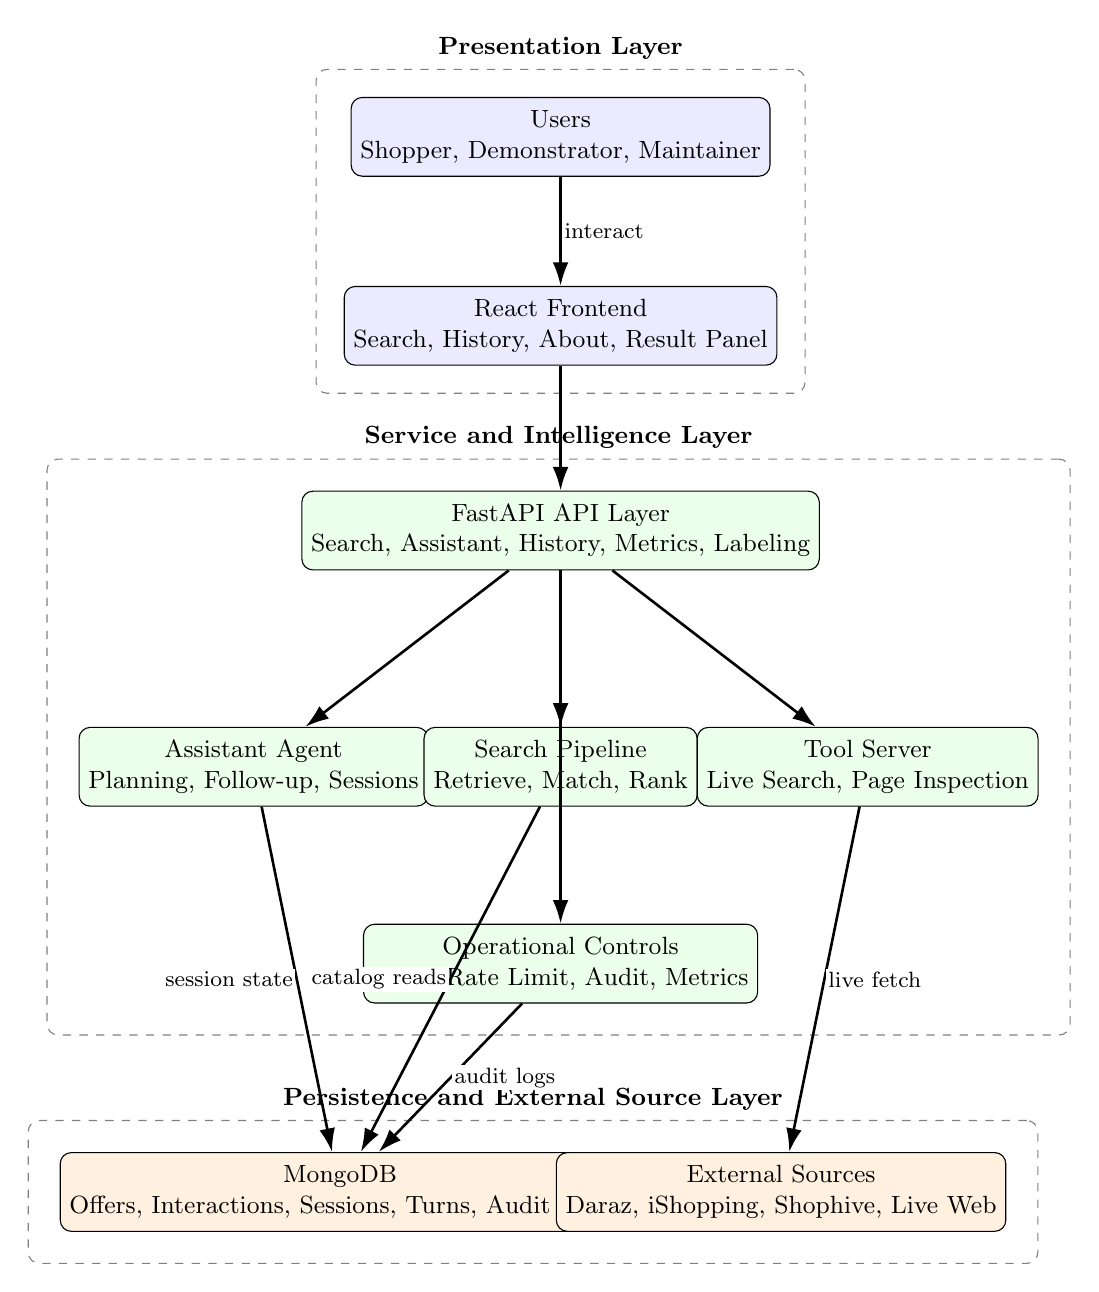
\begin{tikzpicture}[
  font=\small,
  box/.style={draw, rounded corners, align=center, minimum width=5.0cm, minimum height=1.0cm, fill=blue!8},
  service/.style={draw, rounded corners, align=center, minimum width=3.3cm, minimum height=1.0cm, fill=green!8},
  store/.style={draw, rounded corners, align=center, minimum width=4.4cm, minimum height=1.0cm, fill=orange!12},
  arrow/.style={-{Latex[length=3mm,width=2mm]}, line width=0.95pt},
  note/.style={font=\footnotesize, fill=white, inner sep=1pt}
]
\node[box] (users) at (0,9.2) {Users\\Shopper, Demonstrator, Maintainer};
\node[box] (frontend) at (0,6.8) {React Frontend\\Search, History, About, Result Panel};

\node[service] (api) at (0,4.2) {FastAPI API Layer\\Search, Assistant, History, Metrics, Labeling};
\node[service] (assistant) at (-3.9,1.2) {Assistant Agent\\Planning, Follow-up, Sessions};
\node[service] (pipeline) at (0,1.2) {Search Pipeline\\Retrieve, Match, Rank};
\node[service] (tools) at (3.9,1.2) {Tool Server\\Live Search, Page Inspection};

\node[service] (ops) at (0,-1.3) {Operational Controls\\Auth, Rate Limit, Audit, Metrics};

\node[store] (mongo) at (-2.8,-4.2) {MongoDB\\Offers, Interactions, Sessions, Turns, Audit Logs};
\node[store] (web) at (2.8,-4.2) {External Sources\\Daraz, iShopping, Shophive, Live Web};

\draw[arrow] (users) -- node[note,right]{interact} (frontend);
\draw[arrow] (frontend) -- (api);
\draw[arrow] (api) -- (assistant);
\draw[arrow] (api) -- (pipeline);
\draw[arrow] (api) -- (tools);
\draw[arrow] (api) -- (ops);
\draw[arrow] (assistant) -- node[note,left]{session state} (mongo);
\draw[arrow] (pipeline) -- node[note,left]{catalog reads} (mongo);
\draw[arrow] (tools) -- node[note,right]{live fetch} (web);
\draw[arrow] (ops) -- node[note,right]{audit logs} (mongo);

\begin{scope}[on background layer]
\node[draw=black!50, dashed, rounded corners, fit=(users)(frontend), inner sep=0.35cm, label=above:{\textbf{Presentation Layer}}] {};
\node[draw=black!50, dashed, rounded corners, fit=(api)(assistant)(pipeline)(tools)(ops), inner sep=0.4cm, label=above:{\textbf{Service and Intelligence Layer}}] {};
\node[draw=black!50, dashed, rounded corners, fit=(mongo)(web), inner sep=0.4cm, label=above:{\textbf{Persistence and External Source Layer}}] {};
\end{scope}
\end{tikzpicture}
\caption{High-level architecture of the implemented product-search system.}
\label{fig:architecture}
\end{figure}

\section{Design Models}
The following models summarize the runtime behavior and structure of the system. Each diagram is kept portrait-oriented for readability in printed and PDF form.

\subsection{Activity Diagram}

\begin{figure}[H]
\centering
\resizebox{0.70\textwidth}{!}{
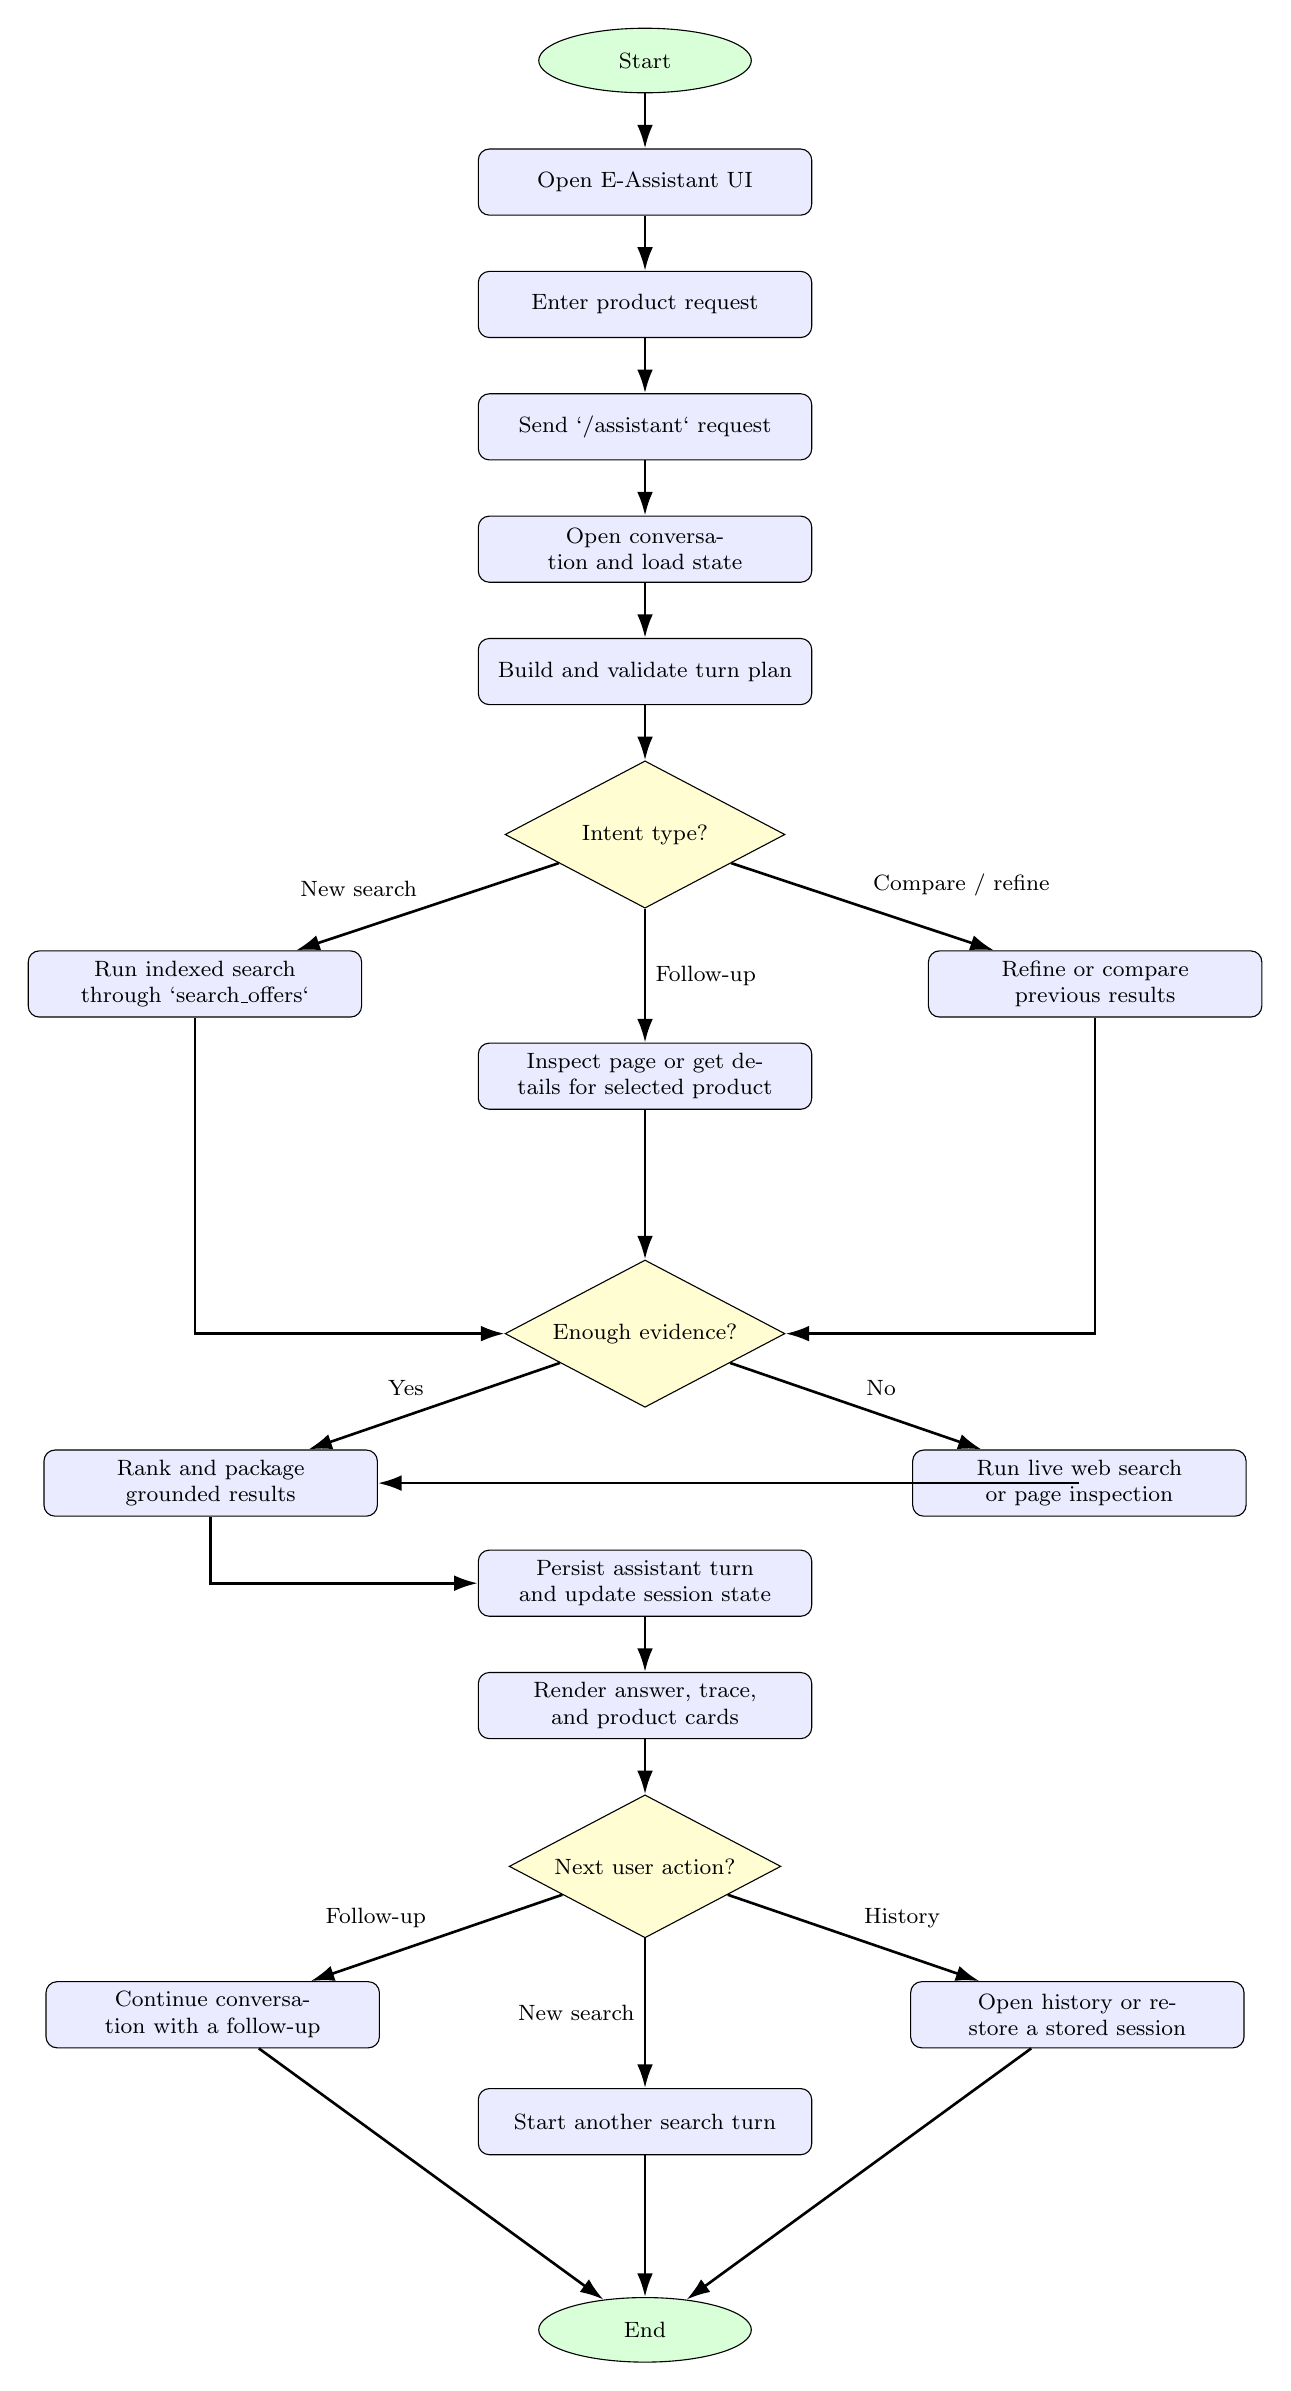
\begin{tikzpicture}[
  font=\footnotesize,
  node distance=0.7cm and 1.0cm,
  action/.style={draw, rounded corners, text width=4.0cm, minimum height=0.84cm, align=center, fill=blue!8},
  decision/.style={draw, diamond, aspect=1.9, text width=2.4cm, align=center, fill=yellow!18},
  terminator/.style={draw, ellipse, minimum width=2.7cm, minimum height=0.82cm, align=center, fill=green!15},
  arrow/.style={-{Latex[length=3mm,width=2mm]}, line width=0.95pt}
]
\node[terminator] (start) {Start};
\node[action, below=of start] (open) {Open E-Assistant UI};
\node[action, below=of open] (query) {Enter product request};
\node[action, below=of query] (submit) {Send `/assistant` request};
\node[action, below=of submit] (memory) {Open conversation and load state};
\node[action, below=of memory] (plan) {Build and validate turn plan};
\node[decision, below=of plan] (intent) {Intent type?};

\node[action, below left=1.0cm and 2.7cm of intent] (newsearch) {Run indexed search through `search\_offers`};
\node[action, below=1.7cm of intent] (followup) {Inspect page or get details for selected product};
\node[action, below right=1.0cm and 2.7cm of intent] (refine) {Refine or compare previous results};

\node[decision, below=1.9cm of followup] (needweb) {Enough evidence?};
\node[action, below left=1.0cm and 2.5cm of needweb] (rank) {Rank and package grounded results};
\node[action, below right=1.0cm and 2.5cm of needweb] (websearch) {Run live web search or page inspection};

\node[action, below=1.8cm of needweb] (persist) {Persist assistant turn and update session state};
\node[action, below=of persist] (display) {Render answer, trace, and product cards};
\node[decision, below=of display] (nextq) {Next user action?};
\node[action, below left=1.0cm and 2.5cm of nextq] (followagain) {Continue conversation with a follow-up};
\node[action, below=1.9cm of nextq] (newturn) {Start another search turn};
\node[action, below right=1.0cm and 2.5cm of nextq] (history) {Open history or restore a stored session};
\node[terminator, below=1.8cm of newturn] (end) {End};

\draw[arrow] (start) -- (open);
\draw[arrow] (open) -- (query);
\draw[arrow] (query) -- (submit);
\draw[arrow] (submit) -- (memory);
\draw[arrow] (memory) -- (plan);
\draw[arrow] (plan) -- (intent);
\draw[arrow] (intent) -- node[above left]{New search} (newsearch);
\draw[arrow] (intent) -- node[right]{Follow-up} (followup);
\draw[arrow] (intent) -- node[above right]{Compare / refine} (refine);
\draw[arrow] (newsearch) |- (needweb);
\draw[arrow] (followup) -- (needweb);
\draw[arrow] (refine) |- (needweb);
\draw[arrow] (needweb) -- node[above left]{Yes} (rank);
\draw[arrow] (needweb) -- node[above right]{No} (websearch);
\draw[arrow] (websearch) |- (rank);
\draw[arrow] (rank) |- (persist);
\draw[arrow] (persist) -- (display);
\draw[arrow] (display) -- (nextq);
\draw[arrow] (nextq) -- node[above left]{Follow-up} (followagain);
\draw[arrow] (nextq) -- node[left]{New search} (newturn);
\draw[arrow] (nextq) -- node[above right]{History} (history);
\draw[arrow] (followagain) -- (end);
\draw[arrow] (newturn) -- (end);
\draw[arrow] (history) -- (end);
\end{tikzpicture}
}
\caption{Activity diagram for conversational product search and follow-up handling.}
\label{fig:activity}
\end{figure}

\subsection{Usecase Diagram}

\begin{figure}[H]
\centering
\resizebox{0.86\textwidth}{!}{
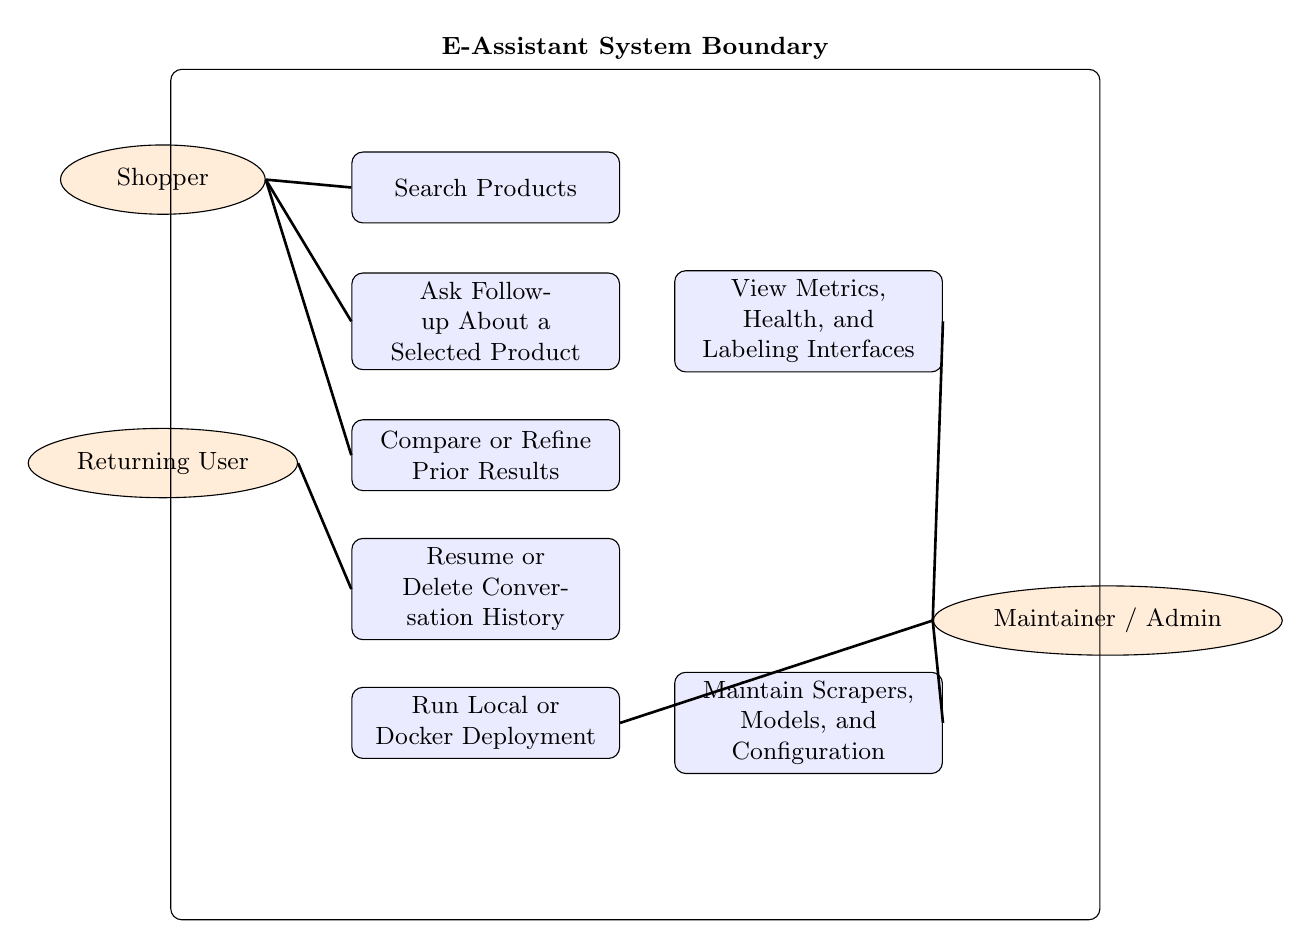
\begin{tikzpicture}[
  font=\small,
  actor/.style={draw, ellipse, minimum width=2.6cm, minimum height=0.88cm, fill=orange!15},
  usecase/.style={draw, rounded corners, text width=2.9cm, minimum width=3.4cm, minimum height=0.9cm, fill=blue!8, align=center},
  arrow/.style={line width=0.95pt}
]
\node[actor] (shopper) at (-6.0,4.2) {Shopper};
\node[actor] (returning) at (-6.0,0.6) {Returning User};
\node[actor] (admin) at (6.0,-1.4) {Maintainer / Admin};

\node[draw, rounded corners, minimum width=11.8cm, minimum height=10.8cm, label=above:{\textbf{E-Assistant System Boundary}}] (boundary) at (0,0.2) {};

\node[usecase] (search) at (-1.9,4.1) {Search Products};
\node[usecase] (followup) at (-1.9,2.4) {Ask Follow-up About a Selected Product};
\node[usecase] (refine) at (-1.9,0.7) {Compare or Refine Prior Results};
\node[usecase] (history) at (-1.9,-1.0) {Resume or Delete Conversation History};
\node[usecase] (deploy) at (-1.9,-2.7) {Run Local or Docker Deployment};
\node[usecase] (metrics) at (2.2,2.4) {View Metrics, Health, and Labeling Interfaces};
\node[usecase] (maintain) at (2.2,-2.7) {Maintain Scrapers, Models, and Configuration};

\draw[arrow] (shopper.east) -- (search.west);
\draw[arrow] (shopper.east) -- (followup.west);
\draw[arrow] (shopper.east) -- (refine.west);
\draw[arrow] (returning.east) -- (history.west);
\draw[arrow] (admin.west) -- (metrics.east);
\draw[arrow] (admin.west) -- (deploy.east);
\draw[arrow] (admin.west) -- (maintain.east);
\end{tikzpicture}
}
\caption{Use case diagram of the implemented product-search system.}
\label{fig:usecase}
\end{figure}

\subsection{Class Diagram}

\begin{figure}[H]
\centering
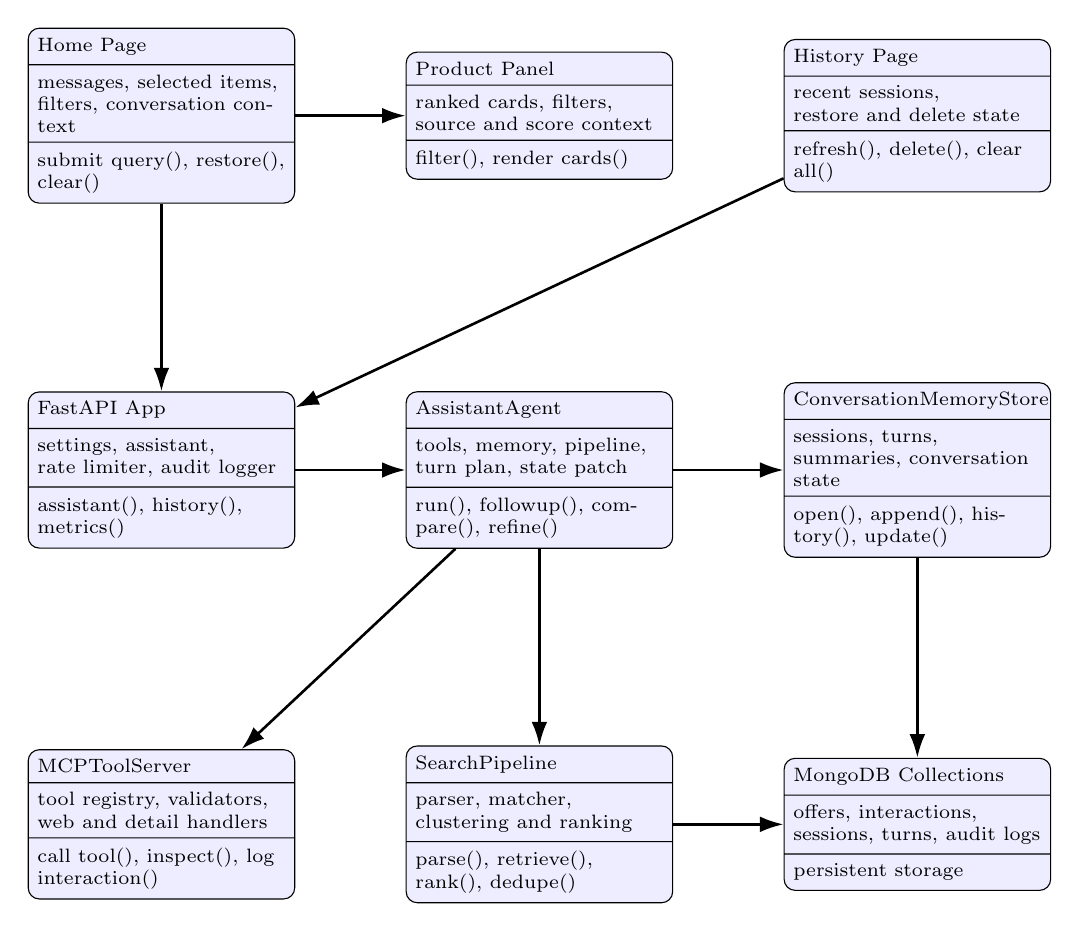
\begin{tikzpicture}[
  font=\scriptsize,
  class/.style={draw, rectangle split, rectangle split parts=3, rounded corners, minimum width=3.15cm, text width=3.15cm, align=left, fill=blue!7},
  arrow/.style={-{Latex[length=3mm,width=2mm]}, line width=0.95pt}
]
\node[class] (home) at (-4.8,6.0) {Home Page\nodepart{second} messages, selected items,\newline filters, conversation context\nodepart{third} submit query(), restore(), clear()};
\node[class] (panel) at (0,6.0) {Product Panel\nodepart{second} ranked cards, filters,\newline source and score context\nodepart{third} filter(), render cards()};
\node[class] (history) at (4.8,6.0) {History Page\nodepart{second} recent sessions,\newline restore and delete state\nodepart{third} refresh(), delete(), clear all()};

\node[class] (apiapp) at (-4.8,1.5) {FastAPI App\nodepart{second} settings, assistant,\newline rate limiter, audit logger\nodepart{third} assistant(), history(), metrics()};
\node[class] (assistant) at (0,1.5) {AssistantAgent\nodepart{second} tools, memory, pipeline,\newline turn plan, state patch\nodepart{third} run(), followup(), compare(), refine()};
\node[class] (memory) at (4.8,1.5) {ConversationMemoryStore\nodepart{second} sessions, turns,\newline summaries, conversation state\nodepart{third} open(), append(), history(), update()};

\node[class] (tools) at (-4.8,-3.0) {MCPToolServer\nodepart{second} tool registry, validators,\newline web and detail handlers\nodepart{third} call tool(), inspect(), log interaction()};
\node[class] (pipeline) at (0,-3.0) {SearchPipeline\nodepart{second} parser, matcher,\newline clustering and ranking\nodepart{third} parse(), retrieve(), rank(), dedupe()};
\node[class] (mongo) at (4.8,-3.0) {MongoDB Collections\nodepart{second} offers, interactions,\newline sessions, turns, audit logs\nodepart{third} persistent storage};

\draw[arrow] (home) -- (panel);
\draw[arrow] (home) -- (apiapp);
\draw[arrow] (history) -- (apiapp);
\draw[arrow] (apiapp) -- (assistant);
\draw[arrow] (assistant) -- (memory);
\draw[arrow] (assistant) -- (tools);
\draw[arrow] (assistant) -- (pipeline);
\draw[arrow] (pipeline) -- (mongo);
\draw[arrow] (memory) -- (mongo);
\end{tikzpicture}
\caption{Conceptual class diagram for the frontend, backend, assistant, and persistence layers.}
\label{fig:class}
\end{figure}

\subsection{Sequence Diagram}

\begin{figure}[H]
\centering
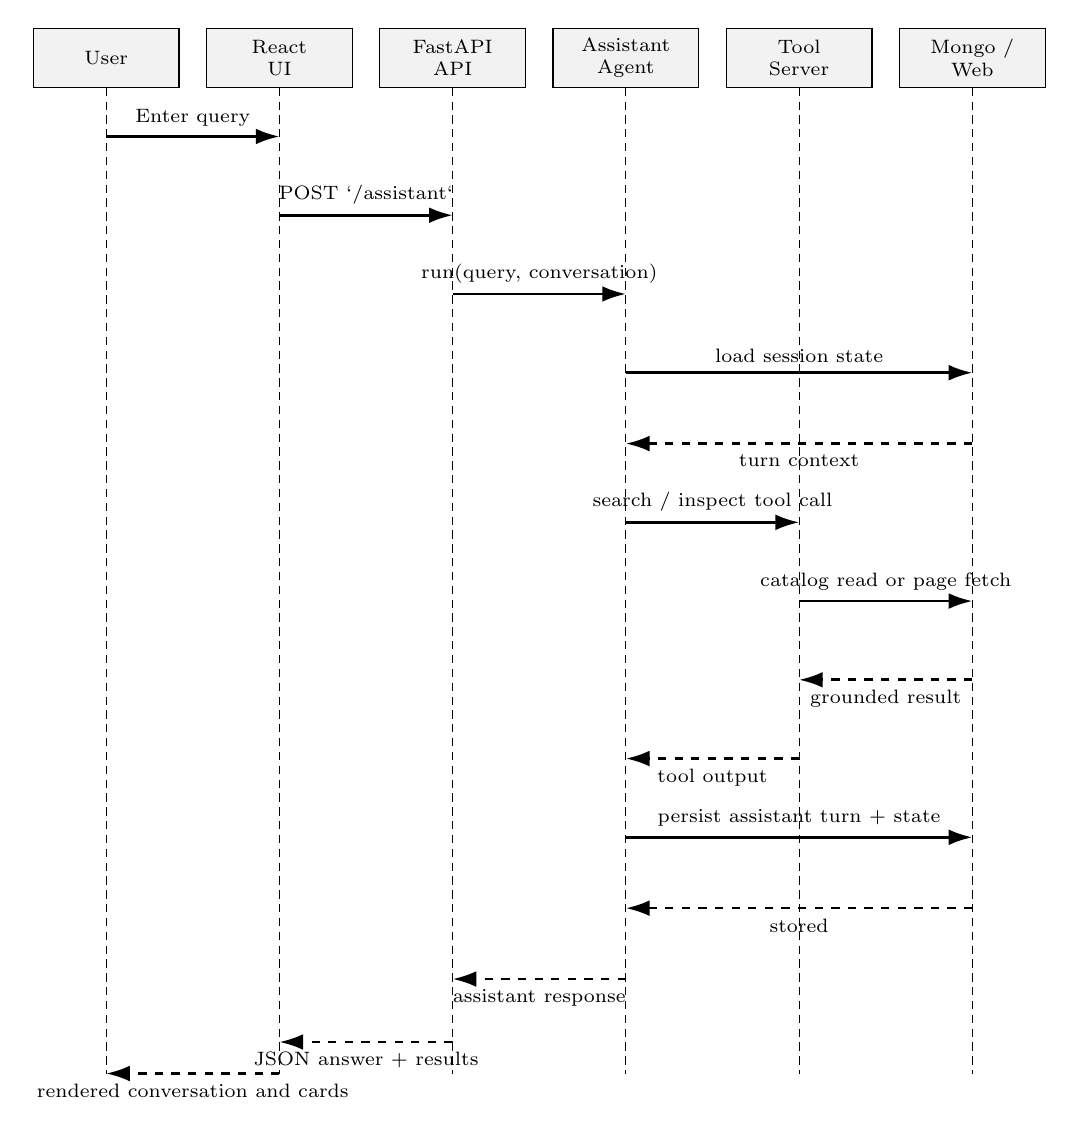
\begin{tikzpicture}[
  font=\scriptsize,
  lifeline/.style={draw, minimum width=1.85cm, minimum height=0.75cm, fill=gray!10, align=center},
  msg/.style={-{Latex[length=3mm,width=2mm]}, line width=0.95pt},
  ret/.style={-{Latex[length=3mm,width=2mm]}, line width=0.95pt, dashed}
]
\node[lifeline] (user) at (0,0) {User};
\node[lifeline] (ui) at (2.2,0) {React\\UI};
\node[lifeline] (api) at (4.4,0) {FastAPI\\API};
\node[lifeline] (agent) at (6.6,0) {Assistant\\Agent};
\node[lifeline] (tools) at (8.8,0) {Tool\\Server};
\node[lifeline] (mongo) at (11.0,0) {Mongo /\\Web};

\foreach \x in {0,2.2,4.4,6.6,8.8,11.0} {
  \draw[densely dashed] (\x,-0.38) -- (\x,-12.9);
}

\draw[msg] (0,-1.0) -- (2.2,-1.0) node[midway,above]{Enter query};
\draw[msg] (2.2,-2.0) -- (4.4,-2.0) node[midway,above]{POST `/assistant`};
\draw[msg] (4.4,-3.0) -- (6.6,-3.0) node[midway,above]{run(query, conversation)};
\draw[msg] (6.6,-4.0) -- (11.0,-4.0) node[midway,above]{load session state};
\draw[ret] (11.0,-4.9) -- (6.6,-4.9) node[midway,below]{turn context};
\draw[msg] (6.6,-5.9) -- (8.8,-5.9) node[midway,above]{search / inspect tool call};
\draw[msg] (8.8,-6.9) -- (11.0,-6.9) node[midway,above]{catalog read or page fetch};
\draw[ret] (11.0,-7.9) -- (8.8,-7.9) node[midway,below]{grounded result};
\draw[ret] (8.8,-8.9) -- (6.6,-8.9) node[midway,below]{tool output};
\draw[msg] (6.6,-9.9) -- (11.0,-9.9) node[midway,above]{persist assistant turn + state};
\draw[ret] (11.0,-10.8) -- (6.6,-10.8) node[midway,below]{stored};
\draw[ret] (6.6,-11.7) -- (4.4,-11.7) node[midway,below]{assistant response};
\draw[ret] (4.4,-12.5) -- (2.2,-12.5) node[midway,below]{JSON answer + results};
\draw[ret] (2.2,-12.9) -- (0,-12.9) node[midway,below]{rendered conversation and cards};
\end{tikzpicture}
\caption{Sequence diagram for an end-to-end assistant search request.}
\label{fig:sequence}
\end{figure}

\subsection{State Transition Diagram}

\begin{figure}[H]
\centering
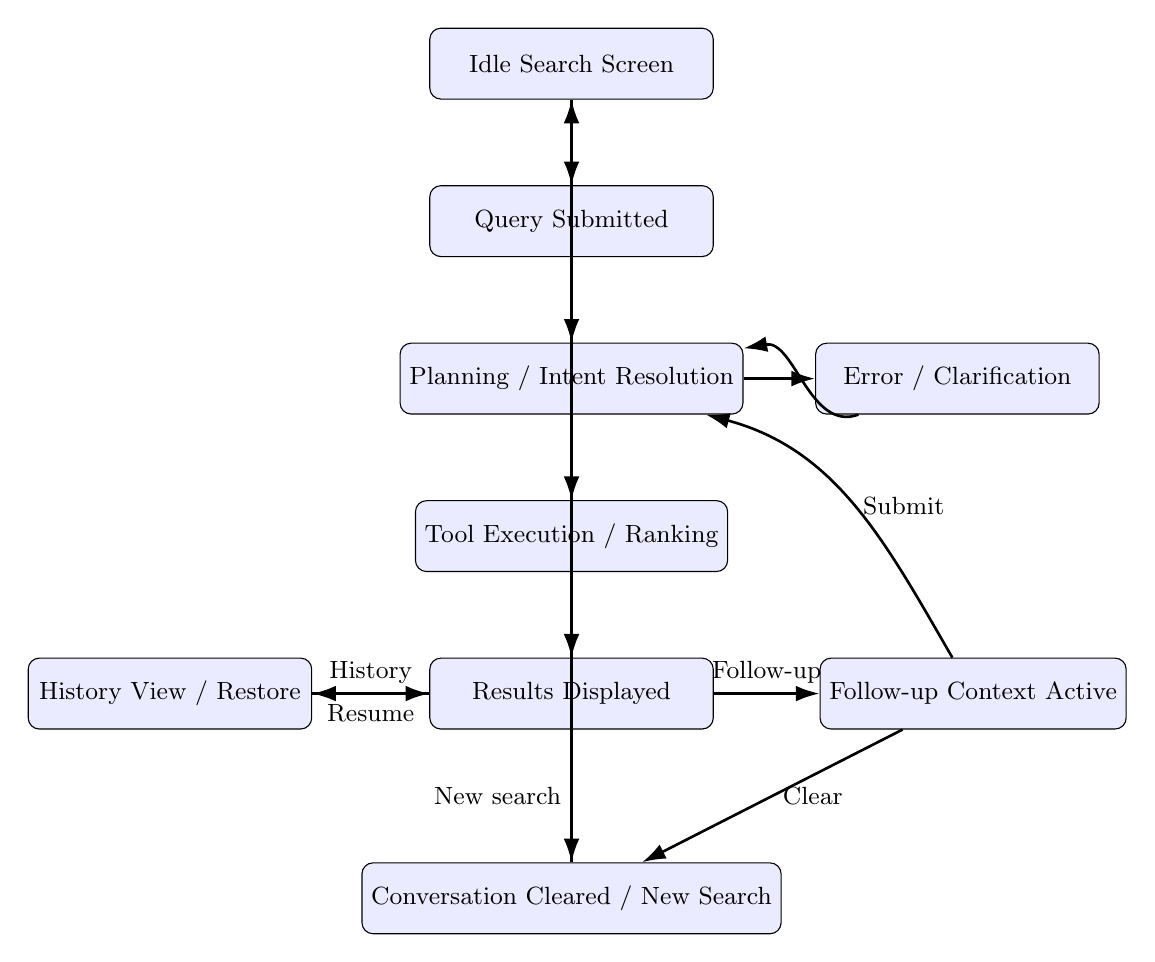
\begin{tikzpicture}[
  font=\small,
  state/.style={draw, rounded corners, minimum width=3.6cm, minimum height=0.9cm, align=center, fill=blue!8},
  arrow/.style={-{Latex[length=3mm,width=2mm]}, line width=0.95pt}
]
\node[state] (idle) at (0,9.0) {Idle Search Screen};
\node[state] (submitted) at (0,7.0) {Query Submitted};
\node[state] (planning) at (0,5.0) {Planning / Intent Resolution};
\node[state] (error) at (4.9,5.0) {Error / Clarification};
\node[state] (tooling) at (0,3.0) {Tool Execution / Ranking};
\node[state] (results) at (0,1.0) {Results Displayed};
\node[state] (history) at (-5.1,1.0) {History View / Restore};
\node[state] (followup) at (5.1,1.0) {Follow-up Context Active};
\node[state] (cleared) at (0,-1.6) {Conversation Cleared / New Search};

\draw[arrow] (idle) -- (submitted);
\draw[arrow] (submitted) -- (planning);
\draw[arrow] (planning) -- (tooling);
\draw[arrow] (planning) -- (error);
\draw[arrow] (error) to[out=200,in=10] (planning);
\draw[arrow] (tooling) -- (results);
\draw[arrow] (results) -- node[above]{History} (history);
\draw[arrow] (history) -- node[below]{Resume} (results);
\draw[arrow] (results) -- node[above]{Follow-up} (followup);
\draw[arrow] (followup) to[out=120,in=-15] node[right]{Submit} (planning);
\draw[arrow] (results) -- node[left]{New search} (cleared);
\draw[arrow] (followup) -- node[right]{Clear} (cleared);
\draw[arrow] (cleared) -- (idle);
\end{tikzpicture}
\caption{State transition diagram for the frontend and assistant interaction flow.}
\label{fig:state}
\end{figure}

\section{Data Design}
The project uses both persistent and transient data.

\textbf{Persistent data} is stored in MongoDB collections. These include raw offers, normalized offers, canonical products, price history, labeled match pairs, user interactions, API audit logs, assistant tool logs, conversation sessions, and conversation turns. Persistent data is what allows the system to operate across runs, preserve user context, and support later training or diagnostics.

\textbf{Transient data} is created during request handling. This includes parsed queries, candidate sets, semantic scores, cluster labels, assistant plans, tool outputs, live web search results, page-inspection outputs, and frontend-rendered result states. These runtime structures are essential to the assistant flow even when they are not permanently stored in full.

\subsection{Data Dictionary}
Tables \ref{tab:collections} and \ref{tab:api-dictionary} summarize the main stored entities and request/response elements.

\begingroup
\small
\setlength{\tabcolsep}{4pt}
\renewcommand{\arraystretch}{1.08}
\begin{longtable}{|L{0.24\textwidth}|L{0.14\textwidth}|L{0.45\textwidth}|}
\caption{Data dictionary for main persistent collections and entities.}\label{tab:collections}\\
\hline
\textbf{Entity} & \textbf{Type} & \textbf{Description} \\
\hline
\endfirsthead
\hline
\textbf{Entity} & \textbf{Type} & \textbf{Description} \\
\hline
\endhead
\textbf{offers\_raw} & Collection & Raw source listings produced by scraper modules before normalization and ranking use. \\
\hline
\textbf{offers\_normalized} & Collection & Searchable normalized product offers with source, price, rating, specifications, stock, and related fields. \\
\hline
\textbf{canonical\_products} & Collection & Higher-level grouped product entities that support cross-offer consolidation. \\
\hline
\textbf{match\_pairs\_labeled} & Collection & Product-pair records used for product-matching evaluation and labeling workflows. \\
\hline
\textbf{user\_interactions} & Collection & Logged events such as view, click, save, and purchase used for personalization support. \\
\hline
\textbf{chat\_sessions} & Collection & Session-level records storing conversation ownership, state, summary, expiry, and next sequence. \\
\hline
\textbf{chat\_turns} & Collection & Turn-level conversation records storing role, content, metadata, timestamp, and expiry. \\
\hline
\textbf{api\_audit\_logs} & Collection & Request audit records that capture method, path, status code, IP, latency, and rate-limit outcome. \\
\hline
\textbf{assistant\_tool\_logs} & Collection / log target & Operational log target for assistant tool activity and debugging information. \\
\hline
\textbf{Model Registry Artifacts} & Filesystem & Active matcher and CF model references selected through the model registry directory. \\
\hline
\end{longtable}
\endgroup

\begingroup
\small
\setlength{\tabcolsep}{4pt}
\renewcommand{\arraystretch}{1.08}
\begin{longtable}{|L{0.22\textwidth}|L{0.14\textwidth}|L{0.47\textwidth}|}
\caption{Data dictionary for assistant and search requests/responses.}\label{tab:api-dictionary}\\
\hline
\textbf{Field} & \textbf{Type} & \textbf{Description} \\
\hline
\endfirsthead
\hline
\textbf{Field} & \textbf{Type} & \textbf{Description} \\
\hline
\endhead
\textbf{Query} & String & Natural-language request submitted by the user through search or assistant endpoints. \\
\hline
\textbf{Conversation ID} & String & Stable identifier for a conversation session used to preserve and restore context. \\
\hline
\textbf{User ID} & String & Browser-level or service-provided user identity used for history and interaction ownership. \\
\hline
\textbf{Top K} & Integer & Result-count limit used in search and assistant requests. \\
\hline
\textbf{Minimum Rating} & Numeric & Optional rating threshold used to bias or filter ranked offers. \\
\hline
\textbf{Assistant Intent} & String & Planned assistant action such as new search, refinement, follow-up, comparison, or clarification. \\
\hline
\textbf{Assistant Context} & Structured data & UI-oriented context describing mode label, selected offer, comparison set, and decision reason. \\
\hline
\textbf{Tool Trace} & Structured data & Optional list of tool calls and high-level outputs returned for frontend inspection. \\
\hline
\textbf{Ranked Result} & Structured data & Offer record containing title, link, source, price, rating, review count, ranking signals, and reason. \\
\hline
\textbf{Interaction Event} & Structured data & Event record containing user, offer, source, link, event type, weight, and timestamp. \\
\hline
\textbf{Page Inspection Output} & Structured data & Extracted signals from a live product page such as rating, review count, shipping, warranty, and availability. \\
\hline
\textbf{Work Log Entry} & Structured data & UI-facing summary of a backend tool invocation shown in the expandable work-log component. \\
\hline
\end{longtable}
\endgroup

\section{Human Interface Design}
The human interface design is based on a clear split between conversation and product evidence. The user does not interact with a generic blank chatbot alone. Instead, the UI keeps search, result ranking, and assistant context visible at the same time. This is an important design choice because shopping support requires both explanation and comparable product cards.

The search page starts with a lightweight welcome state, source-status pills, quick prompts, and a single input field. Once the user submits a query, the conversation pane shows the assistant's grounded answer while the result panel displays product cards, ranking badges, filters, and context chips. This allows the system to support both question answering and browsing without forcing the user to switch between separate screens for every step.

The history page is intentionally simple. It shows recent sessions, timestamps, result counts, and resume/delete actions. This matches the actual browser-storage-based session model used in the implementation. The page does not present complex account settings because the current system is not built around full authenticated user accounts.

The about page works as an informational product surface. It explains the platform idea, feature themes, and value proposition. In architectural terms it is secondary to the search workflow, but it is useful for demonstration because it gives evaluators a quick overview of what the platform is intended to do.

\section{Algorithm}
The runtime logic can be described in two related algorithms: indexed conversational search and selected-product follow-up.

\textbf{Indexed conversational search algorithm}
\begin{enumerate}[leftmargin=0.35in]
    \item Receive a natural-language request at the frontend and send it to the `/assistant` endpoint with the current conversation ID and user ID.
    \item Open or create the conversation session and load recent turns and stored state from MongoDB.
    \item Build a turn plan that classifies the request as a new search, refinement, comparison, selected-product follow-up, clarification-needed state, or general question.
    \item If the request is a new search, parse the query and retrieve indexed candidates from `offers\_normalized` using text search and filters.
    \item Apply relevance filtering, semantic query-to-candidate matching, clustering, value-oriented reranking, and optional collaborative-filtering score blending.
    \item If indexed coverage is weak or if live evidence is required, call live web search and/or page inspection tools.
    \item Build a grounded response and product result set from tool outputs rather than from unsupported generated content.
    \item Persist the assistant turn, compact result preview, assistant context, and updated session state in MongoDB.
    \item Return the answer, results, and optional tool trace to the frontend for rendering.
\end{enumerate}

\textbf{Selected-product follow-up algorithm}
\begin{enumerate}[leftmargin=0.35in]
    \item Detect that the current user message refers to an earlier result or an active selected product.
    \item Resolve the referenced product from stored conversation state or prior result indexes.
    \item Retrieve saved normalized offer details and inspect the product page when delivery, availability, warranty, specs, price, or review evidence is needed.
    \item Merge trusted stored and inspected signals while rejecting obvious listing-page misreads or price outliers.
    \item Generate a grounded answer focused on the requested aspect, such as delivery, review strength, or comparison verdict.
    \item Persist the new assistant turn and update the active product state for the next follow-up.
\end{enumerate}

\section{Tools and Technologies}
The system combines multiple frameworks across frontend, backend, data, and intelligence layers.

\begin{table}[H]
\centering
\small
\setlength{\tabcolsep}{4pt}
\renewcommand{\arraystretch}{1.08}
\caption{Tools and technologies used in the implemented product-search system.}
\label{tab:tools}
\begin{tabular}{|L{0.21\textwidth}|L{0.24\textwidth}|L{0.40\textwidth}|}
\hline
\textbf{Layer} & \textbf{Technology} & \textbf{Purpose in the Project} \\
\hline
Frontend & React, TypeScript, Vite, React Router & Search UI, history page, navigation, component-based rendering, and local development server. \\
\hline
Frontend interaction & Framer Motion, Lucide React & Motion effects, UI transitions, and icon-based interface elements. \\
\hline
Backend API & FastAPI, Uvicorn, Pydantic & Request validation, routing, service hosting, and API contracts. \\
\hline
Database & MongoDB, PyMongo & Storage for normalized offers, sessions, turns, interactions, audit logs, and labeling data. \\
\hline
Assistant runtime & Python orchestration layer & Turn planning, clarification logic, follow-up handling, comparison flow, refinement flow, and context persistence. \\
\hline
Search and ranking & Sentence-transformer-style matcher, clustering, reranking, CF utilities & Semantic retrieval support, product grouping, ranking, and personalization blending. \\
\hline
Web extraction & Playwright, Requests, Beautiful Soup & Scraping configured sources and inspecting product pages for live signals. \\
\hline
LLM services & Groq-backed model calls & Query parsing, assistant JSON planning, and live web search support when enabled. \\
\hline
Supplementary UI & Gradio & Optional lightweight demonstration and testing interface. \\
\hline
Deployment & Python runner, Docker, Docker Compose & Local orchestration and containerized service startup. \\
\hline
\end{tabular}
\end{table}

\section{User Interface}
The UI section documents the implemented E-Assistant frontend through screenshots stored in the project's documentation folder. The screenshots cover the dashboard-like landing state, the result-rich search state, the history page, and the about page.

\uitwoscreenshots{"UI screenshots/Dashboard.png"}{"UI screenshots/Product search.png"}

\subsection{Main Search and Result Workflow}
The first screenshot page shows the search dashboard in both its initial and active states. The initial state emphasizes the branded entry point, quick prompts, and the main search box. The active result state shows how the conversation pane, assistant context chips, and ranked product panel work together once a search has been executed. This reflects the core product workflow of the system.

\uitwoscreenshots{"UI screenshots/History.png"}{"UI screenshots/About.png"}

\subsection{History and About Screens}
The second screenshot page shows the history page and the about page. The history page demonstrates session restoration and deletion support for earlier searches. The about page provides a concise explanatory view of the platform's purpose and feature highlights. Together, these screens complete the main user-facing structure of the application.

\section{Deployment}
The project is deployed as a lightweight multi-service application. The primary demonstration path starts a FastAPI backend and a Vite frontend together through the local runner. MongoDB provides the persistent data layer, and an optional Docker Compose stack is available for containerized execution.

The local deployment path is centered around `run\_all.py`. This script resolves the frontend toolchain, optionally installs dependencies, starts the API, waits for the health endpoint to become ready, and then launches the React frontend with the appropriate proxy target. This makes local project evaluation straightforward.

The container deployment path is defined through `docker-compose.yml`. It provisions MongoDB, builds the API container, and builds the frontend container. The web service exposes the interface through port 3000 while the API remains available on port 8000. This is sufficient for demonstration and review even though it is not intended as a production-scale deployment model.

\begin{table}[H]
\centering
\small
\setlength{\tabcolsep}{4pt}
\renewcommand{\arraystretch}{1.08}
\caption{Deployment environment summary.}
\label{tab:deployment-summary}
\begin{tabular}{|L{0.20\textwidth}|L{0.16\textwidth}|L{0.18\textwidth}|L{0.32\textwidth}|}
\hline
\textbf{Component} & \textbf{Runtime} & \textbf{Deployment Role} & \textbf{Purpose} \\
\hline
React Frontend & Node.js / Vite or Nginx container & Presentation service & Provides search, history, about, and ranked-result UI. \\
\hline
FastAPI Backend & Python / Uvicorn & Intelligence and API service & Exposes assistant, search, recommendation, history, metrics, and labeling endpoints. \\
\hline
MongoDB & MongoDB service & Persistence layer & Stores offers, sessions, turns, interactions, audit logs, and related project data. \\
\hline
Gradio Interface & Python / Gradio & Supplementary interface & Provides an alternative lightweight demonstration entry point. \\
\hline
Docker Compose & Docker runtime & Deployment orchestration & Starts web, API, and MongoDB services together for containerized execution. \\
\hline
\end{tabular}
\end{table}

\begin{table}[H]
\centering
\small
\setlength{\tabcolsep}{4pt}
\renewcommand{\arraystretch}{1.08}
\caption{Deployment components and configuration detail.}
\label{tab:deployment-components}
\begin{tabular}{|L{0.28\textwidth}|L{0.56\textwidth}|}
\hline
\textbf{Deployment Item} & \textbf{Detail} \\
\hline
Environment configuration & `.env` defines Mongo URI, API keys, model settings, rate limits, and live search behavior. \\
\hline
Local startup runner & `run\_all.py` starts the API first, waits for health readiness, then launches the frontend with the correct proxy target. \\
\hline
API startup & The backend is served through `uvicorn src.api.app:app` with configurable host and port. \\
\hline
Frontend startup & The React app runs through `npm run dev` for development or through the built container path in Docker deployment. \\
\hline
Mongo dependency & MongoDB is required for offer storage, conversation persistence, interactions, and audit records. \\
\hline
Operational controls & Authorization mode, rate-limiter backend, metrics exposure, and live web behavior are all configuration-driven. \\
\hline
Container deployment & Docker Compose provisions Mongo, API, and web services with health dependencies between them. \\
\hline
\end{tabular}
\end{table}

Operationally, the system is suitable for classroom evaluation, local demonstration, and controlled project testing. Before any broader public deployment, the project would still require stronger operational hardening, source-governance controls, secret handling, and more formal monitoring of scraping and live inspection reliability.

\section{Chapter Summary}
This chapter documented the implemented system from design and architecture perspectives. It defined the major modules, explained the layered runtime structure, and provided diagrams for workflow, actors, classes, sequences, and states. It also described the data design, human interface, core algorithms, toolchain, screenshots, and deployment model. Together, these sections show how the project functions as a complete AI-powered product-search application.

\begin{thebibliography}{99}

\bibitem{reimers2019}
Nils Reimers and Iryna Gurevych.
\newblock Sentence-BERT: Sentence embeddings using Siamese BERT-networks.
\newblock In \emph{Proceedings of the 2019 Conference on Empirical Methods in Natural Language Processing}, 2019.

\bibitem{fastapi}
Sebastian Ramirez.
\newblock FastAPI documentation.
\newblock \url{https://fastapi.tiangolo.com/}

\bibitem{mongodb}
MongoDB.
\newblock MongoDB documentation.
\newblock \url{https://www.mongodb.com/docs/}

\bibitem{react}
React.
\newblock React documentation.
\newblock \url{https://react.dev/}

\bibitem{vite}
Vite.
\newblock Vite documentation.
\newblock \url{https://vite.dev/}

\bibitem{playwrightdocs}
Microsoft.
\newblock Playwright documentation.
\newblock \url{https://playwright.dev/}

\bibitem{bs4docs}
Beautiful Soup.
\newblock Beautiful Soup documentation.
\newblock \url{https://www.crummy.com/software/BeautifulSoup/bs4/doc/}

\bibitem{gradio}
Gradio.
\newblock Gradio documentation.
\newblock \url{https://www.gradio.app/docs}

\end{thebibliography}

\end{document}
